\MDNAME\
%%%%%%%%%%%%%%%%%%%%%%%%%%%%%%%%%%%%%%%%%%%%%%%%%%%%%%%%%%%%%%%%%%%%%%%%%%%%%%%
% DO NOT MODIFY THIS FILE
%%%%%%%%%%%%%%%%%%%%%%%%%%%%%%%%%%%%%%%%%%%%%%%%%%%%%%%%%%%%%%%%%%%%%%%%%%%%%%%

\section{Easy Plug}

Copied from:

\begin{itemize}
\item
  http://wiki.keyestudio.com/index.php/Ks0099\_keyestudio\_EASY\_plug\_Control\_Board
\end{itemize}

Keyestudio Easy-plug control board is a microcontroller board based on
the ATmega328P-PU. It has 14 digital input/outputs (of which 6 can be
used as PWM outputs), 6 analog inputs, a 16 MHz quartz crystal, a USB
connection, a power jack, an ICSP header and a reset button. It contains
everything needed to support the microcontroller; simply connect it to a
computer with a USB cable or power it with a AC-to-DC adapter or battery
to get started.You can tinker with your UNO without worrying too much
about doing something wrong, worst case scenario you can replace the
chip for a few dollars and start over again. For convenience of wire
connection, we simplify pins GND and VCC into each plug, so you only
need one wire to connect a module, no need to separately connect the VCC
and GND. The pins on the original UNO are all redesigned into plug
interface. On the board, you can find ports D2-D13, A0 to A5, an IIC
port and a COM port. All in one simple plug.

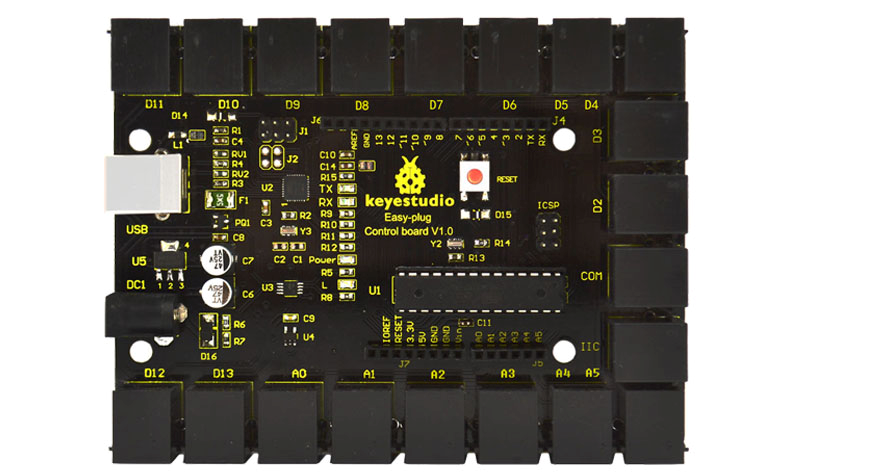
\includegraphics[width=0.8\columnwidth]{images/easyplug.png}

\subsection{Specifications}

\begin{longtable}[]{@{}ll@{}}
\toprule
Microcontroller core & ATmega328P-PU\tabularnewline
\midrule
\endhead
Working voltage & +5V\tabularnewline
External input voltage & \(+7V - +12V\) (suggested)\tabularnewline
External input voltage (externum) &
\(+6V \leq Vin \leq +20V\)\tabularnewline
Digital signal I/O interface & 14 (of which 6 provide PWM
output)\tabularnewline
Analog signal input interface & 6\tabularnewline
DCI/O interface current & 20 mA\tabularnewline
FlashMemory & 32KB (ATmega328) of which 0.5 KB used by
bootloader\tabularnewline
SRAM static storage capacity & 2KB\tabularnewline
EEPROM storage capacity & 1 KB\tabularnewline
EEPROM storage capacity & 16 MHz\tabularnewline
\bottomrule
\end{longtable}

\subsection{Connect}

Tools -\textgreater{} Arduino/Genuin Arduino

port oon OSX will loock something like this:

\begin{itemize}
\item
  /dev/cu.usbmodem1461
\end{itemize}

\subsection{Test code}

\begin{lstlisting}
int command;
int port;

int pin_from = 5;
int pin_to = 13;

void Light(int pin){
  digitalWrite(pin,HIGH);
  delay(500);
  digitalWrite(pin,LOW);
}

void setup() {
  Serial.begin(9600);
  int i;
  for (i = pin_from; i <= pin_to; i++){
    pinMode(i,OUTPUT);
  }
}


void loop() {
 command=Serial.read();
  if(command=='a') {
    int i;
    for (i = pin_from; i <= pin_to; i++){
      Light(i);    
      Serial.print("Led ");
      Serial.println(i);
      delay(100);
    }
  }
}
\end{lstlisting}

\subsection{Kit List}

\begin{itemize}
\item
  http://www.keyestudio.com/keyestudio-easy-plug-learning-kit-for-arduino-super-makers.html
\end{itemize}

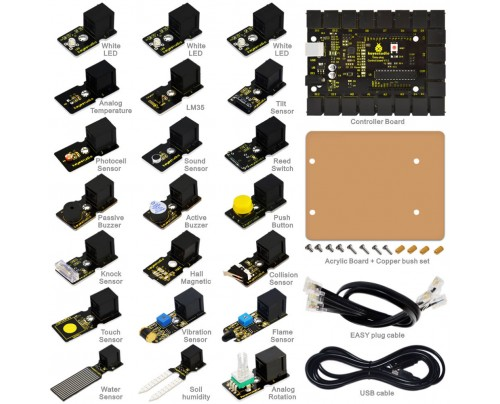
\includegraphics[width=0.8\columnwidth]{images/easyplugkit.jpg}

\begin{longtable}[]{@{}ll@{}}
\toprule
Part & Number\tabularnewline
\midrule
\endhead
EASY plug controller Board & 1\tabularnewline
Acrylic Board + Copper bush set & 1\tabularnewline
EASY plug cable & 3\tabularnewline
USB cable & 1\tabularnewline
EASY plug Piranha LED Module & 3\tabularnewline
EASY plug Line Tracking Sensor & 1\tabularnewline
EASY plug Infrared obstacle avoidance sensor & 1\tabularnewline
EASY plug Photo Interrupter Module & 1\tabularnewline
EASY plug PIR Motion Sensor & 1\tabularnewline
EASY plug DS18B20 Temperature Sensor & 1\tabularnewline
EASY plug IR Receiver Module & 1\tabularnewline
EASY plug IR Transmitter Module & 1\tabularnewline
EASY plug Single Relay Module & 1\tabularnewline
EASY plug ADXL345 Three Axis Acceleration Module & 1\tabularnewline
EASY plug DHT11 Temperature and Humidity Sensor & 1\tabularnewline
EASY plug DS3231 Clock Module & 1\tabularnewline
EASY plug Analog Gas Sensor & 1\tabularnewline
EASY plug Analog Alcohol Sensor & 1\tabularnewline
EASY plug MQ135 Air Quality Sensor & 1\tabularnewline
EASY plug BMP180 Barometric Pressure Sensor & 1\tabularnewline
EASY plug Bluetooth Module & 1\tabularnewline
EASY plug 1602 I2C Module & 1\tabularnewline
EASY plug I2C 8x8 LED Matrix & 1\tabularnewline
\bottomrule
\end{longtable}

\subsection{Command Language}

on PORT

\begin{itemize}
\item
  switches PORT on
\end{itemize}

off PORT

\begin{itemize}
\item
  switches port off
\end{itemize}

on all

\begin{itemize}
\item
  switches all ports on
\end{itemize}

off all

\begin{itemize}
\item
  switches all ports off
\end{itemize}

dance

\begin{itemize}
\item
  goes serially through ports and switches them on and off
\end{itemize}

\begin{lstlisting}
String command;


int pin_from = 5;
int pin_to = 13;

String getValue(String data, char separator, int index)
{
  // copied from internet
    int found = 0;
    int strIndex[] = { 0, -1 };
    int maxIndex = data.length() - 1;

    for (int i = 0; i <= maxIndex && found <= index; i++) {
        if (data.charAt(i) == separator || i == maxIndex) {
            found++;
            strIndex[0] = strIndex[1] + 1;
            strIndex[1] = (i == maxIndex) ? i+1 : i;
        }
    }
    return found > index ? data.substring(strIndex[0], strIndex[1]) : "";
}

void Light(int pin, int action){
  if (action ==  1) {
    digitalWrite(pin,HIGH);
  } else {
    digitalWrite(pin,LOW);
  }
}

void wait_for_input() {
  while (Serial.available()==0) { } 
}

void setup() {
  Serial.begin(9600);
  int i;
  for (i = pin_from; i <= pin_to; i++){
    pinMode(i,OUTPUT);
  }
}


void loop() {
 
  Serial.print("command:");
  wait_for_input();
  command=Serial.readString();  
  Serial.println (command);

   if (command=="dance") {     
      for (int i = pin_from; i <= pin_to; i++) {
        Light(i,1);
        delay(100);
        Light(i,0);    
        Serial.print("Led ");
        Serial.println(i);
        delay(100);
      }
    } else {
      
      int action;
      String action_name = getValue(command, ' ', 0);
      String port_name = getValue(command, ' ', 1);

      action = action_name == "on";
    
      if (port_name == "all") {
        for (int i = pin_from; i <= pin_to; i++){
          Light(i,action);   
          Serial.print("Led ");
          Serial.println(i);
        }
      } else {
        int port = port_name.toInt();

        Serial.println(action);
        Serial.println(port);
        Light(port, action);
     }
  }
}
\end{lstlisting}

